\documentclass[aspectratio=1610]{beamer}

\usepackage{amsmath}
\usepackage{multirow}
\usepackage{url}
\usepackage{hyperref}

\hypersetup{
colorlinks=false,
}

\usepackage{listings,calc,graphicx}

\title % [short title] (optional, use only with long paper titles)
{CPSC 1000: Introduction to Computer Science}

\subtitle{Week 2: generating digital signals} % (optional)

\author{Robert Benkoczi, C556\\\url{robert.benkoczi@uleth.ca}}
\date{18-Sep-2018}

% for figures created with IPE
%\pdfpagebox5

\lstloadlanguages{C}
\lstset{language=C,tabsize=2,aboveskip=-22pt,belowskip=-22pt,keepspaces,
  basicstyle=\small\ttfamily,}


\begin{document}

\begin{frame}[plain]
\titlepage
\end{frame}

%%%%%%

\begin{frame}[t,plain]{Week 1 lecture objectives}
To prepare students for lab activity 1: Arduino's digital
output. Digital output is needed for the functioning of various
electronic components, such as the ultrasonic distance sensor.

\begin{itemize}
\item Students will examine the different pins of an Arduino
  micro-controller. 
\item Students will write a simple program for the Arduino to generate
  a digital signal.
\item Students will assemble a simple electronic circuit using a
  breadboard to visualize the digital signal.
\end{itemize}
\end{frame}


%%%%%%

\begin{frame}[plain]{An Arduino and its pins}

\begin{center}
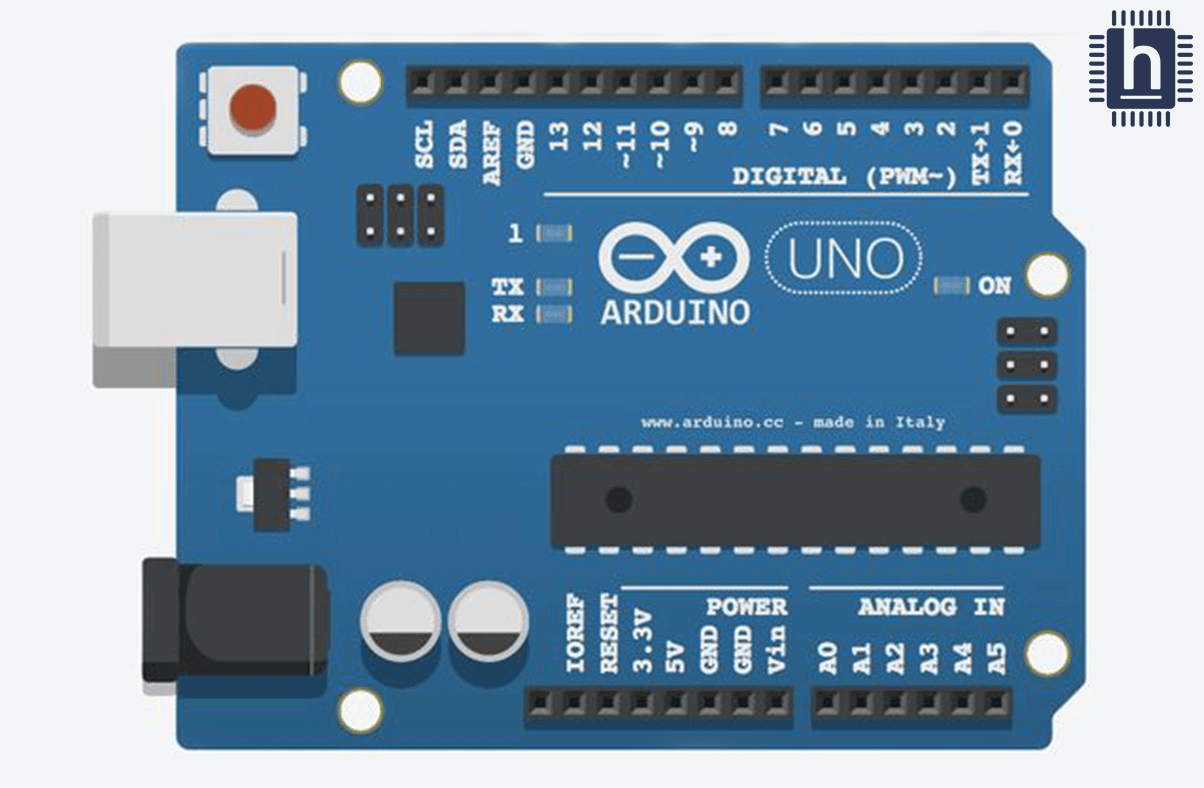
\includegraphics[width=0.5\textwidth]{figs/1-arduino-simple.png}
\end{center}
\end{frame}


%%%%%%

\begin{frame}[plain,t]{Breadboard}

  Hobbyists used breadboards to test electronic circuit prototypes.
 

\begin{center}
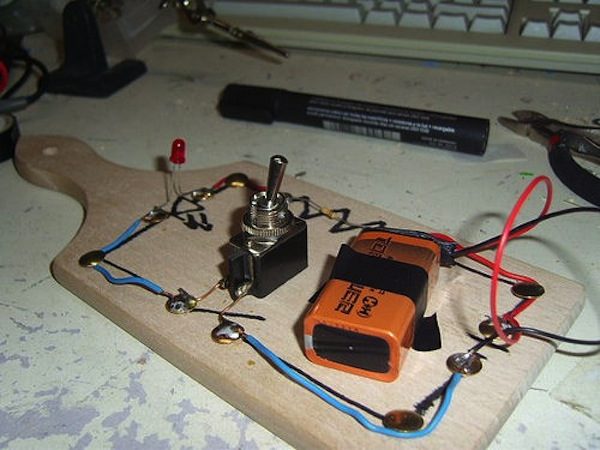
\includegraphics[width=.6\textwidth]{figs/1-bread.jpg}
\end{center}
\end{frame}


%%%%%%

\begin{frame}[plain,t]{The breadboard we will use}

\begin{center}
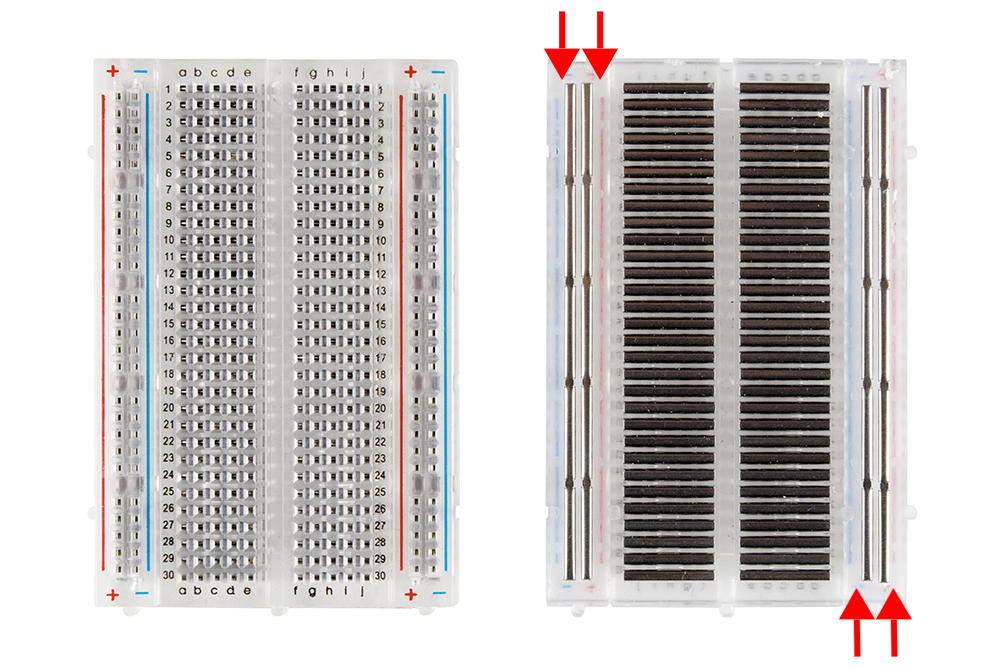
\includegraphics[width=.9\textwidth]{figs/1-breadboard.jpg}
\end{center}
\end{frame}


%%%%%%

\begin{frame}[plain,t]{Example}
Connect two resistors in parallel

\bigskip
\begin{center}
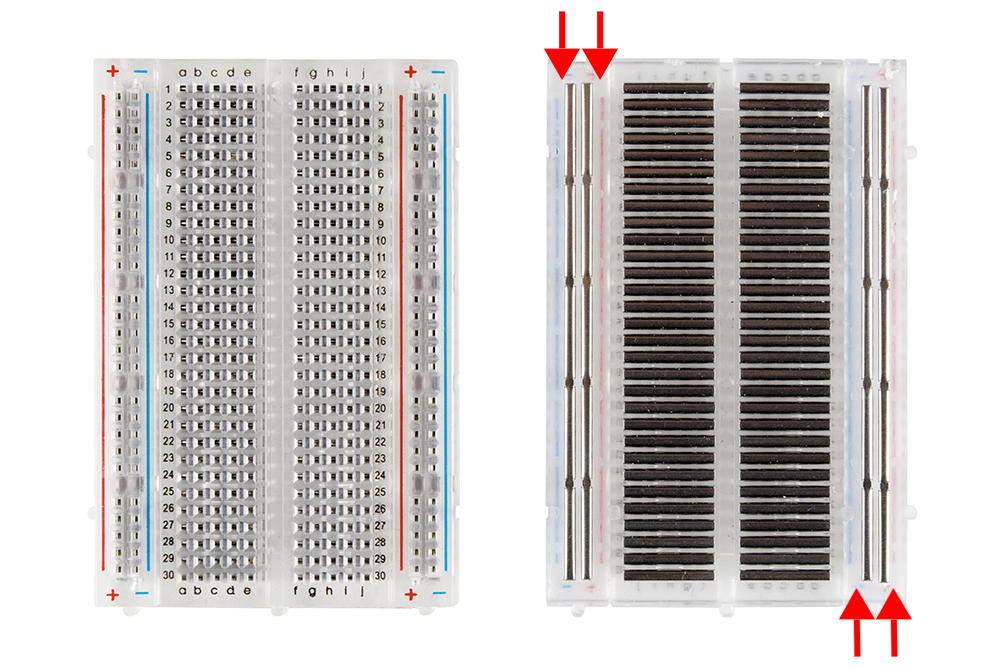
\includegraphics[width=.9\textwidth]{figs/1-breadboard.jpg}
\end{center}
\end{frame}

%%%%%%

\begin{frame}[plain,t]{Exercises}

\begin{itemize}
\item Two resistors in series.
\item Two resistors in parallel, connected in series with one
  resistor.
\item Two parallel resistors in series with other two parallel
  resistors.
\item Two series resistors, in parallel with other two series resistors.
\end{itemize}

\bigskip
\begin{center}
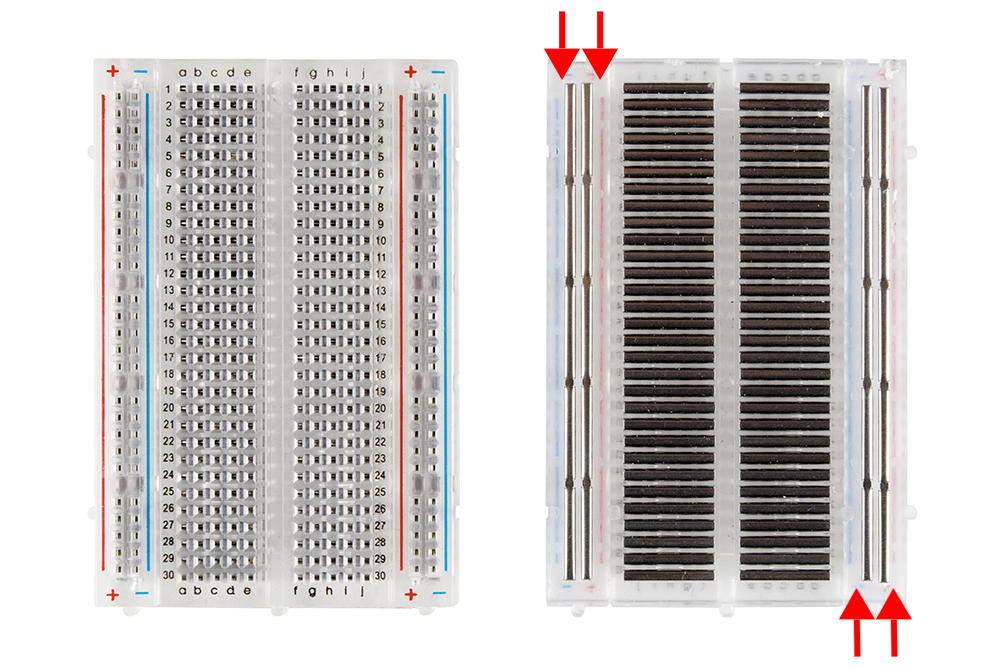
\includegraphics[width=.7\textwidth]{figs/1-breadboard.jpg}
\end{center}
\end{frame}


%%%%%%

\begin{frame}[plain,t]{Diodes}
\begin{itemize}
\item Current flows only in one direction (in the opposite direction
  the current is very small, ``reverse current'').
\item There is voltage in the forward direction, ``forward voltage''.
\item There is a max current in forward direction (higher current can
  damage the LED).
\item There is a max voltage in the reverse direction, ``breakdown voltage''.
\end{itemize}
\end{frame}


%%%%%%

\begin{frame}[plain,t]{Using an LED with the arduino, Ohm,'s Law}
\begin{itemize}
\item Max current out of an Arduino's digital pin: 40 mA (also note
  the LED's max forward current).
\item Bit 1 represented as +5 V. 
\item Forward voltage on a LED, eg: 2.5 V.
\item $U = I \cdot R$, $I$: current (intensity), $R$: resistance, $U$:
  voltage.
\end{itemize}
\end{frame}


%%%%%%
\begin{frame}[plain,t]{Programming the Arduino to generate digital signals}

  \medskip
  Digital signal:
  \parbox[t]{3cm}{
    \begin{itemize}
      \item 0V = bit 0
      \item 5V = bit 1.
  \end{itemize}}

  \medskip
  Arduino digital pins:
  \parbox[t]{6cm}{
    \begin{itemize}
      \item Input = measuring device
      \item Output = battery
  \end{itemize}}
  
\end{frame}


%%%%%%

\begin{frame}[plain,t,fragile]{Setting up the digital pin for input/output}

Function \texttt{pinMode}:

\bigskip
Example:
\begin{semiverbatim}
\begin{lstlisting}
void setup()
{
  pinMode(13, OUTPUT);
}
\end{lstlisting}
\end{semiverbatim}
\end{frame}


%%%%%%


\begin{frame}[plain,t,fragile]{Generating bit 1 or bit 0}

  Function \texttt{digitalWrite}

\bigskip
Example:
\begin{semiverbatim}
\begin{lstlisting}  
void loop()
{
  digitalWrite(13, HIGH);
  delay(1000); // Wait for 1000 millisecond(s)
  digitalWrite(13, LOW);
  delay(1000); // Wait for 1000 millisecond(s)
}
\end{lstlisting}
\end{semiverbatim}
\end{frame}


%%%%%%%

\begin{frame}[plain,t]{Make the LED blink twice in a second}

\end{frame}


%%%%%%%

\begin{frame}[plain,t]{Program a long blink followed by a short blink}


\end{frame}

%%%%%%%


\end{document}
